\documentclass[a4paper,12pt]{article}
\usepackage[utf8]{inputenc}
\usepackage[T1]{fontenc}
\usepackage[english]{babel}
\usepackage{color}
\usepackage{lmodern}
\usepackage{amsmath}
\usepackage{amssymb}
\usepackage{amsthm}
\usepackage{mathtools}
\usepackage[superscript]{cite}
\usepackage{listings}
\usepackage[ruled, linesnumbered, longend]{algorithm2e}
\usepackage{dsfont}
\usepackage{nicefrac}
\usepackage{upgreek}
\usepackage{paralist}
\usepackage{tabulary}
\usepackage{stmaryrd}
\usepackage{tikz}
\usepackage{pgffor}
\usepackage{pgfplots}
\usepackage{graphicx}
\usepackage{setspace}
\usepackage{fancyhdr}
% \usepackage[colorlinks=true,linkcolor=blue]{hyperref}				% Blue hyperlinks look better than red boxed ones

% Header
\newcommand\shorttitle{}
\newcommand\authors{Dominik Blank}

\fancyhf{} % sets all head and foot elements empty
\fancyhead[L]{\shorttitle}
\fancyhead[R]{\authors}
\fancyfoot[C]{\thepage}
\pagestyle{fancy} % sets the page style to the style delivered and editable with fancyhdr

% Own commands, operators, etc.
\newcommand{\abs}[1]{\lvert#1\rvert}
\newcommand{\norm}[1]{\lVert#1\rVert}

% Math environments
\theoremstyle{plain}
\newtheorem{theorem}{Theorem}[section]
\newtheorem{lemma}[theorem]{Lemma}
\newtheorem{corollary}[theorem]{Corollary}
\theoremstyle{definition}
\newtheorem{definition}[theorem]{Definition}
\newtheorem{notation}[theorem]{Notation}
\newtheorem{remark}[theorem]{Remark}
\newtheorem{example}[theorem]{Example}

% END PREAMBLE

\author{Dominik Blank}
\title{On the influence of morphological operators on testing for a region of interest}

\onehalfspacing
\setlength{\parindent}{0pt}
\allowdisplaybreaks

\begin{document}

\begin{theorem}
	Let $m, n \in \mathbb{N}$, $c \in \mathbb{R} \setminus \{ 0 \}$ and $\Omega = \left\{ 1, \dots, m \right\} \times \left\{ 1, \dots, n \right\}$.
	
	Assume that $F$ follows the statistical model given in \eqref{image} and let $T(i, j)$ be the test statistic as defined in \eqref{teststatistic} and $H_1(i, j)$ be the alternative hypothesis as defined in \eqref{alternativehypothesis}. Let $t$ be a threshold, such that
	\begin{equation*}
		\mathbb{P}_V\left( T(i, j) \leq t \right) \leq \beta
	\end{equation*}
	for all $V \in \mathcal{H}_1(i, j)$. Let $\mathfrak{I}$ be the binary image defined by
	\begin{equation}
		\mathfrak{I}(i, j) = \mathds{1}_{ \{ T(i, j) \geq t \} }
	\end{equation}
	for all $(i, j) \in \Omega$.
	
	Let $\varphi \in \mathbb{N}$ be odd. Let $\Phi_\varphi = \{ -\frac{\varphi - 1}{2}, -\frac{\varphi - 3}{2}, \dots, \frac{\varphi - 3}{2}, \frac{\varphi - 1}{2} \}$ and $\Psi_\varphi = \Phi_\varphi \times \Phi_\varphi$ be a structuring element. Let $(i, j) \in \Omega$ and $V \in \mathcal{H}_1(i, j)$.
	
	Denote by $\varLambda = \{ \kappa_1, \dots, \kappa_2 \} \times \{ \lambda_1, \dots, \lambda_2 \}$ the rROI contained in $V$. Let $\min \{ \kappa_2 - \kappa_1 + 1, \lambda_2 - \lambda_1 + 1 \} \geq \varphi$.
	Then the following inequalities hold:
	\begin{align}
		\mathbb{P}_V( (\mathfrak{I} \circ \Psi_\varphi)(i, j) = 0 ) &\leq \varphi^2 \beta \label{ineqtypeIIopening} \\
		\mathbb{P}_V( ((\mathfrak{I} \circ \Psi_\varphi) \bullet \Psi_\varphi)(i, j) = 0 ) &\leq \varphi^2 \beta \label{ineqtypeIIclosing}
	\end{align}
\end{theorem}
\begin{proof}
	We use $\Psi_\varphi = \Phi_\varphi \times \Phi_\varphi$ and get
	\begin{align*}
		\mathbb{P}&_V( ((\mathfrak{I} \circ \Psi_\varphi) \bullet \Psi_\varphi)(i, j) = 0 ) \\
		&= \mathbb{P}_V\left( \bigcup_{(k, l) \in \Psi_\varphi} \bigcap_{(\tilde{k}, \tilde{l}) \in \Psi_\varphi} \bigcap_{(r, s) \in \Psi_\varphi} \bigcup_{(\tilde{r}, \tilde{s}) \in \Psi_\varphi} \{ \mathfrak{I}(i + k - \tilde{k} - r + \tilde{r}, j + l - \tilde{l} - s + \tilde{s}) = 0 \} \right) \\
		&= \mathbb{P}_V\left( \bigcup_{k, l \in \Phi_\varphi} \bigcap_{\tilde{k}, \tilde{l} \in \Phi_\varphi} \bigcap_{r, s \in \Phi_\varphi} \bigcup_{\tilde{r}, \tilde{s} \in \Phi_\varphi} \{ \mathfrak{I}(i + k - \tilde{k} - r + \tilde{r}, j + l - \tilde{l} - s + \tilde{s}) = 0 \} \right)
	\end{align*}
	
	Using sub-additivity we obtain
	\begin{align*}
		\mathbb{P}&_V( ((\mathfrak{I} \circ \Psi_\varphi) \bullet \Psi_\varphi)(i, j) = 0 ) \\
		&= \mathbb{P}_V\left( \bigcup_{k, l \in \Phi_\varphi} \bigcap_{\tilde{k}, \tilde{l} \in \Phi_\varphi} \bigcap_{r, s \in \Phi_\varphi} \bigcup_{\tilde{r}, \tilde{s} \in \Phi_\varphi} \{ \mathfrak{I}(i + k - \tilde{k} - r + \tilde{r}, j + l - \tilde{l} - s + \tilde{s}) = 0 \} \right) \\
		&\leq \sum_{k, l \in \Phi_\varphi} \mathbb{P}_V\left( \bigcap_{\tilde{k}, \tilde{l} \in \Phi_\varphi} \bigcap_{r, s \in \Phi_\varphi} \bigcup_{\tilde{r}, \tilde{s} \in \Phi_\varphi} \{ \mathfrak{I}(i + k - \tilde{k} - r + \tilde{r}, j + l - \tilde{l} - s + \tilde{s}) = 0 \} \right)
	\end{align*}
	
	We can pull the two intersections together and get
	\begin{align*}
		\mathbb{P}&_V( ((\mathfrak{I} \circ \Psi_\varphi) \bullet \Psi_\varphi)(i, j) = 0 ) \\
		&\leq \sum_{k, l \in \Phi_\varphi} \mathbb{P}_V\left( \bigcap_{\tilde{k}, \tilde{l} \in \Phi_\varphi} \bigcap_{r, s \in \Phi_\varphi} \bigcup_{\tilde{r}, \tilde{s} \in \Phi_\varphi} \{ \mathfrak{I}(i + k - \tilde{k} - r + \tilde{r}, j + l - \tilde{l} - s + \tilde{s}) = 0 \} \right) \\
		&= \sum_{k, l \in \Phi_\varphi} \mathbb{P}_V\left( \bigcap_{\tilde{k}, \tilde{l}, r, s \in \Phi_\varphi} \bigcup_{\tilde{r}, \tilde{s} \in \Phi_\varphi} \{ \mathfrak{I}(i + k - \tilde{k} - r + \tilde{r}, j + l - \tilde{l} - s + \tilde{s}) = 0 \} \right)
	\end{align*}
	
	We drop every term in the intersection besides $r - \tilde{k}, s - \tilde{l} \in \{ - ( \varphi - 1 ), \varphi - 1 \}$. This yields
	\begin{align*}
		\mathbb{P}&_V( ((\mathfrak{I} \circ \Psi_\varphi) \bullet \Psi_\varphi)(i, j) = 0 ) \\
		&\leq \sum_{k, l \in \Phi_\varphi} \mathbb{P}_V\left( \bigcap_{\tilde{k}, \tilde{l}, r, s \in \Phi_\varphi} \bigcup_{\tilde{r}, \tilde{s} \in \Phi_\varphi} \{ \mathfrak{I}(i + k - \tilde{k} - r + \tilde{r}, j + l - \tilde{l} - s + \tilde{s}) = 0 \} \right) \\
		&\leq \sum_{k, l \in \Phi_\varphi} \mathbb{P}_V\left( \bigcap_{r - \tilde{k}, s - \tilde{l} \in \{ - ( \varphi - 1 ), \varphi - 1 \}} \bigcup_{\tilde{r}, \tilde{s} \in \Phi_\varphi} \{ \mathfrak{I}(i + k - \tilde{k} - r + \tilde{r}, j + l - \tilde{l} - s + \tilde{s}) = 0 \} \right)
	\end{align*}
	
	The sets $\bigcup_{\tilde{r}, \tilde{s} \in \Phi_\varphi} \{ \mathfrak{I}(i + k - \tilde{k} - r + \tilde{r}, j + l - \tilde{l} - s + \tilde{s}) = 0 \}$ are mutually independent for $r - \tilde{k}, s - \tilde{l} \in \{ - ( \varphi - 1 ), \varphi - 1 \}$ and fixed $k, l \in \Phi_\varphi$. Thus we obtain
	\begin{align*}
		\mathbb{P}&_V( ((\mathfrak{I} \circ \Psi_\varphi) \bullet \Psi_\varphi)(i, j) = 0 ) \\
		&\leq \sum_{k, l \in \Phi_\varphi} \mathbb{P}_V\left( \bigcap_{r - \tilde{k}, s - \tilde{l} \in \{ - ( \varphi - 1 ), \varphi - 1 \}} \bigcup_{\tilde{r}, \tilde{s} \in \Phi_\varphi} \{ \mathfrak{I}(i + k - \tilde{k} - r + \tilde{r}, j + l - \tilde{l} - s + \tilde{s}) = 0 \} \right) \\
		&= \sum_{k, l \in \Phi_\varphi} \prod_{r - \tilde{k}, s - \tilde{l} \in \{ - ( \varphi - 1 ), \varphi - 1 \}} \mathbb{P}_V\left( \bigcup_{\tilde{r}, \tilde{s} \in \Phi_\varphi} \{ \mathfrak{I}(i + k - \tilde{k} - r + \tilde{r}, j + l - \tilde{l} - s + \tilde{s}) = 0 \} \right)
	\end{align*}
	
	Again, by using sub-additivy, we get
	\begin{align*}
		\mathbb{P}&_V( ((\mathfrak{I} \circ \Psi_\varphi) \bullet \Psi_\varphi)(i, j) = 0 ) \\
		&\leq \sum_{k, l \in \Phi_\varphi} \prod_{r - \tilde{k}, s - \tilde{l} \in \{ - ( \varphi - 1 ), \varphi - 1 \}} \mathbb{P}_V\left( \bigcup_{\tilde{r}, \tilde{s} \in \Phi_\varphi} \{ \mathfrak{I}(i + k - \tilde{k} - r + \tilde{r}, j + l - \tilde{l} - s + \tilde{s}) = 0 \} \right) \\
		&= \sum_{k, l \in \Phi_\varphi} \prod_{r - \tilde{k}, s - \tilde{l} \in \{ - ( \varphi - 1 ), \varphi - 1 \}} \sum_{\tilde{r}, \tilde{s} \in \Phi_\varphi} \mathbb{P}_V\left( \{ \mathfrak{I}(i + k - \tilde{k} - r + \tilde{r}, j + l - \tilde{l} - s + \tilde{s}) = 0 \} \right)
	\end{align*}
	
	Using the assumption $\mathbb{P}_V\left( T(i, j) \leq t \right) \leq \beta$ we obtain the upper bound
	\begin{align*}
		\mathbb{P}&_V( ((\mathfrak{I} \circ \Psi_\varphi) \bullet \Psi_\varphi)(i, j) = 0 ) \\
		&\leq \sum_{k, l \in \Phi_\varphi} \prod_{r - \tilde{k}, s - \tilde{l} \in \{ - ( \varphi - 1 ), \varphi - 1 \}} \sum_{\tilde{r}, \tilde{s} \in \Phi_\varphi} \mathbb{P}_V\left( \{ \mathfrak{I}(i + k - \tilde{k} - r + \tilde{r}, j + l - \tilde{l} - s + \tilde{s}) = 0 \} \right) \\
		&\leq \sum_{k, l \in \Phi_\varphi} \prod_{r - \tilde{k}, s - \tilde{l} \in \{ - ( \varphi - 1 ), \varphi - 1 \}} \sum_{\tilde{r}, \tilde{s} \in \Phi_\varphi} \beta \\
		&= \sum_{k, l \in \Phi_\varphi} \prod_{r - \tilde{k}, s - \tilde{l} \in \{ - ( \varphi - 1 ), \varphi - 1 \}} \varphi^2 \beta \\
		&= \sum_{k, l \in \Phi_\varphi} ( \varphi^2 \beta )^4 \\
		&= \varphi^2 ( \varphi^2 \beta )^4 \\
		&= \varphi^{10} \beta^4
	\end{align*}
	
	This finishes the proof.
\end{proof}

\newpage

\begin{figure}[h]
	\centering
	\resizebox{\textwidth}{!}{
		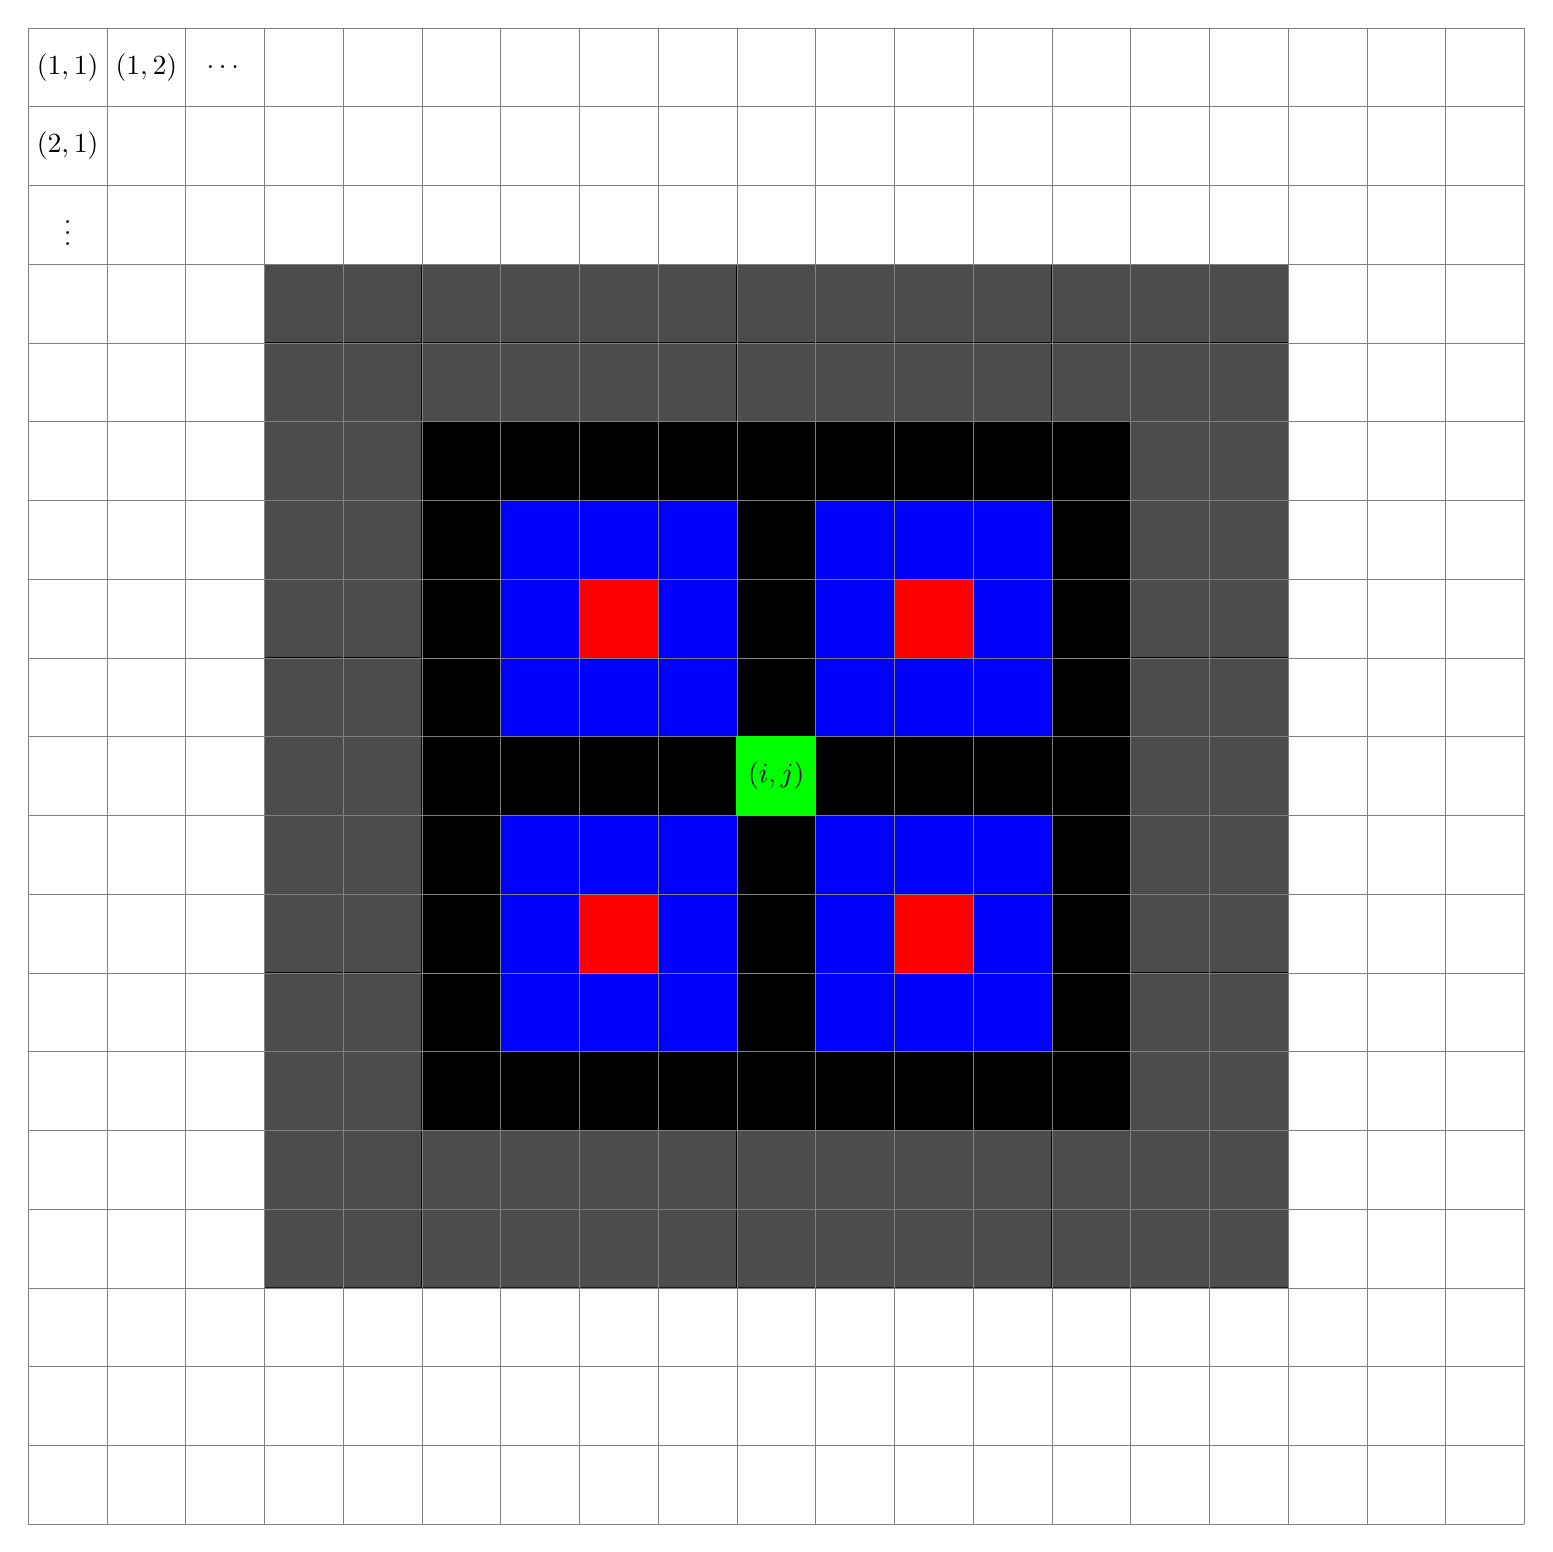
\begin{tikzpicture}
			\foreach \i in {-6, ..., 6}
				\foreach \j in {-6, ..., 6}
					\filldraw[black, opacity=0.7] (\i, \j) rectangle + (1, 1);
			\foreach \i in {-4, ..., 4}
				\foreach \j in {-4, ..., 4}
					\filldraw[black] (\i, \j) rectangle + (1, 1);
			\foreach \x in {(-3, -3), (-3, 1), (1, -3), (1, 1)}
				\filldraw[blue] \x rectangle + (3, 3);
			\foreach \x in {(-2, -2), (-2, 2), (2, -2), (2, 2)}
				\filldraw[red] \x rectangle + (1, 1);
			\draw[help lines, step=1] (-9, -9) grid (10, 10);
			\filldraw[green] (0, 0) rectangle + (1, 1);
			\node at (0.5, 0.5) {$(i, j)$};
			\node at (-8.5, 9.5) {$(1, 1)$};
			\node at (-7.5, 9.5) {$(1, 2)$};
			\node at (-6.5, 9.5) {$\dots$};
			\node at (-8.5, 8.5) {$(2, 1)$};
			\node at (-8.5, 7.5) {$\vdots$};
		\end{tikzpicture}
	}
	\caption{The black area is the pixels that contribute to $(\mathfrak{I} \circ \Psi_\varphi) \bullet \Psi_\varphi)(i, j)$. The blue squares are mutually independent. The red pixels are the pixels that we reduce the intersection in the proof to.}
	\label{powerindependentpoints}
\end{figure}


\end{document}
